% !TEX encoding = UTF-8 Unicode
% !TEX TS-program = pdflatex
% !TEX spellcheck = it-IT
\documentclass[a4paper,titlepage]{article}

\usepackage[utf8x]{inputenc}
\usepackage{hyperref}

\makeatletter
\def\input@path{{../documenti/template/}} %uso i template usati finora
\makeatother

\usepackage{Comandi}
\usepackage{Riferimenti}
\usepackage{Stile}

%Nome del documento
\def\NOME{Documento per Miriade}
%Versione del documento
\def\VERSIONE{1.0.0}
%Data del documento
\def\DATA{2016-09-14}
%Redattore/i del documento. Va scritto prima il nome, poi il cognome
\def\REDATTORE{Andrea Grendene}
%Verificatore del documento
\def\VERIFICATORE{}
%Responsabile del \gl{progetto}
\def\RESPONSABILE{}
%Destinatari del documento
\def\DESTINATARI{\PROPONENTE}

%Sommario del documento
\def\SOMMARIO{Questo documento ha lo scopo di presentare tutti i dati richiesti da \PROPONENTE\ per il progetto del gruppo \AUTORE.}

\begin{document}

\maketitle

	% le ultime modifiche vanno messe in testa alla tabella
\begin{diario} %TODO: valutare se inserire un nuovo comando per il diario senza il ruolo
	\modifica{Andrea Grendene}{\PRJ}{Creata struttura base del documento}{2016-09-14}{0.0.1}
\end{diario}

\newpage
\tableofcontents
\newpage
\listoftables
\newpage
\listoffigures

\section{Prove effettuate}
\label{prove}
%Qui inseriremo le prove effettuate con il nostra progetto, insieme all'elenco dei beacon utilizzati, alla loro disposizione, al loro scopo e ai loro dati. Sar� infine aggiunta una valutazione dell'esito della prova.
Durante la realizzazione di questo progetto sono stati effettuati alcuni test per verificare che tutto il sistema funzionasse correttamente. In questa sezione essi verranno descritti, in particolare per quanto riguarda la disposizione e le impostazioni dei beacon, insieme all'esito finale e ai problemi da risolvere sorti durante la loro esecuzione.
	\subsection{Percorso di prova ufficiale della Revisione di Accettazione}
		Non � un test ma un percorso ufficiale vero e proprio, � stato aggiunto in questa sezione perch� l'esito ottenuto ha portato a individuare dei miglioramenti da implementare per il percorso finale.
		Il percorso consiste in 3 stazioni da giocare nell'edificio Torre Archimede dell'Universit� degli Studi di Padova. La partenza, ovvero quando viene premuto il pulsante di inizio percorso, � al primo piano nell'aula 1C150, mentre la prima tappa � situata vicino all'entrata della biblioteca, al primo piano interrato. All'inizio quindi � stato verificato che i beacon della altre tappe vengono scartati quando sono rilevati. Giocata la prima tappa il percorso prevede che l'utente torni per la stessa strada della partenza, stavolta per� pu� giocare le altre tappe, visto che vengono rilevati in ordine i beacon della seconda e della terza tappa.
	
		\begin{tabella}{!{\VRule}l!{\VRule}l!{\VRule}l!{\VRule}} %TODO: aggiungere dati dispositivo usato
			\intestazionethreecol{Nome dispositivo}{Versione Android}{Note sull'esito della prova}
			LG Nexus 5x & 7.0 & \\
			\caption{Tabella con i dati dei dispositivi usati per il percorso}
		\end{tabella}
	
		\subsubsection{Dati e disposizione dei beacon}
		L'UUID di tutti i beacon � \textbf{f7826da6-4fa2-4e98-8024-bc5b71e0893e}.
	
		\begin{figure}[!h]
				\centering
				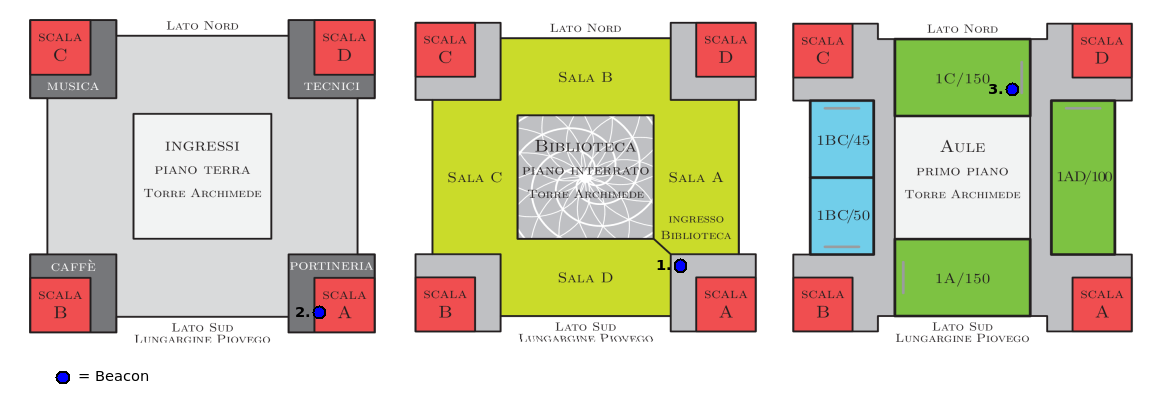
\includegraphics[scale=0.4]{planimetrie/TorreArchimede}  
				\caption{Planimetria della Torre Archimede con la posizione dei beacon segnata}
		\end{figure}
	
		\begin{tabella}{!{\VRule}l!{\VRule}l!{\VRule}l!{\VRule}l!{\VRule}l!{\VRule}l!{\VRule}}
			\intestazionesixcol{Numero beacon}{Major}{Minor}{Potenza (dBm)}{Intervallo (ms)}{Note posizione}
			1. & 0 & 0 & -20 & 150 & \\
			2. & 1 & 0 & -12 & 150 & Beacon posizionato davanti a una finestra della scala. � richiesta pi� potenza per coprire tutta l'area \\
			3. & 2 & 0 & -20 & 150 & \\
			\caption{Tabella con i dati dei beacon usati per il percorso}
		\end{tabella}
	
		\subsubsection{Esito della prova}
		La prova ha avuto successo, all'andata sono stati esclusi i beacon delle altre tappe e al ritorno sono stati rilevati in un tempo accettabile, inoltre le funzioni mostrate sono state eseguite come previsto.
		A seguito di questa prova e dei test eseguiti in precedenza per la sua preparazione abbiamo individuato delle modifiche abbastanza importanti da apportare, come l'aggiunta delle proximity, ovvero le interfacce che, quando rilevano un determinato beacon, comunicano all'utente quanto manca per raggiungere la prossima stazione, oppure un miglioramento della gestione degli errori che possono essere restituiti dal server.
	\subsection{Test sul funzionamento delle Proximity}
		In questo test � stato verificato che le classi relative al funzionamento delle Proximity funzionassero correttamente. Per eseguire il test abbiamo preso quattro beacon, due per le prime due prove del percorso e due per due proximity presenti tra la prima e la seconda prova. Il percorso usato � quello preparato per la Revisione di Accettazione, ma sono stati usati solo una parte dei beacon necessari, quindi esso non � stato portato a termine.
	
		\begin{tabella}{!{\VRule}l!{\VRule}l!{\VRule}l!{\VRule}}
			\intestazionethreecol{Nome dispositivo}{Versione Android}{Note sull'esito della prova}
			LG Nexus 5x & 7.0 & \\
			Motorola Moto G & 5.0 & \\
			\caption{Tabella con i dati dei dispositivi usati per il percorso}
		\end{tabella}
	
		\subsubsection{Dati e disposizione dei beacon}
		I beacon sono stati disposti lungo un corridoio dritto in Torre Archimede, quindi seguendo una linea retta. Pi� precisamente sono stati posati sul davanzale interno all'edificio, quindi a circa 110 cm di altezza. \\
		
		L'UUID di tutti i beacon � \textbf{f7826da6-4fa2-4e98-8024-bc5b71e0893e}.
	
		\begin{tabella}{!{\VRule}l!{\VRule}l!{\VRule}l!{\VRule}l!{\VRule}l!{\VRule}l!{\VRule}}
			\intestazionesixcol{Numero beacon}{Major}{Minor}{Potenza (dBm)}{Intervallo (ms)}{Note posizione}
			1. & 0 & 0 & -30 & 150 & \\
			2. & 5 & 0 & -30 & 150 & \\
			3. & 4 & 0 & -30 & 150 & \\
			4. & 1 & 0 & -30 & 150 & \\
			\caption{Tabella con i dati dei beacon usati per il percorso}
		\end{tabella}
	
		\subsubsection{Esito della prova}
		La prova ha avuto successo, anche se sono stati rilevati degli errori nelle classi da verificare, prontamente risolti al momento. La cosa forse pi� preoccupante � la difficolt� nel gestire il raggio massimo in cui il beacon pu� essere rilevato, anche se probabilmente era dovuto all'errore nelle classi delle Proximity. Si vedr� durante la prova del percorso per Miriade se riscontreremo ancora problemi di questo tipo.
	\label{prova_percorso_Miriade}
	\subsection{Test generale del percorso per Miriade}
		In questo test � stato verificato che il percorso da presentare a Miriade il 30 settembre funzionasse correttamente, oltre a impostare la potenza dei beacon pi� adatta alla loro posizione.
	
		\begin{tabella}{!{\VRule}l!{\VRule}l!{\VRule}l!{\VRule}}
			\intestazionethreecol{Nome dispositivo}{Versione Android}{Note sull'esito della prova}
			LG G3 & 5.0 & Ci mette parecchio tempo a rilevare i beacon, come distanza invece � nella media \\
			LG Nexus 5x & 7.0 & La rilevazione dei beacon avviene ad una distanza superiore rispetto alla media \\
			Motorola Moto G & 5.0 & \\
			\caption{Tabella con i dati dei dispositivi usati per il percorso}
		\end{tabella}
	
		\subsubsection{Dati e disposizione dei beacon}
		I primi 8 beacon sono quelli delle stazioni, i rimanenti invece sono usati dalle proximity. \\
		
		L'UUID di tutti i beacon � \textbf{f7826da6-4fa2-4e98-8024-bc5b71e0893e}.
		
		\begin{figure}[!h]
				\centering
				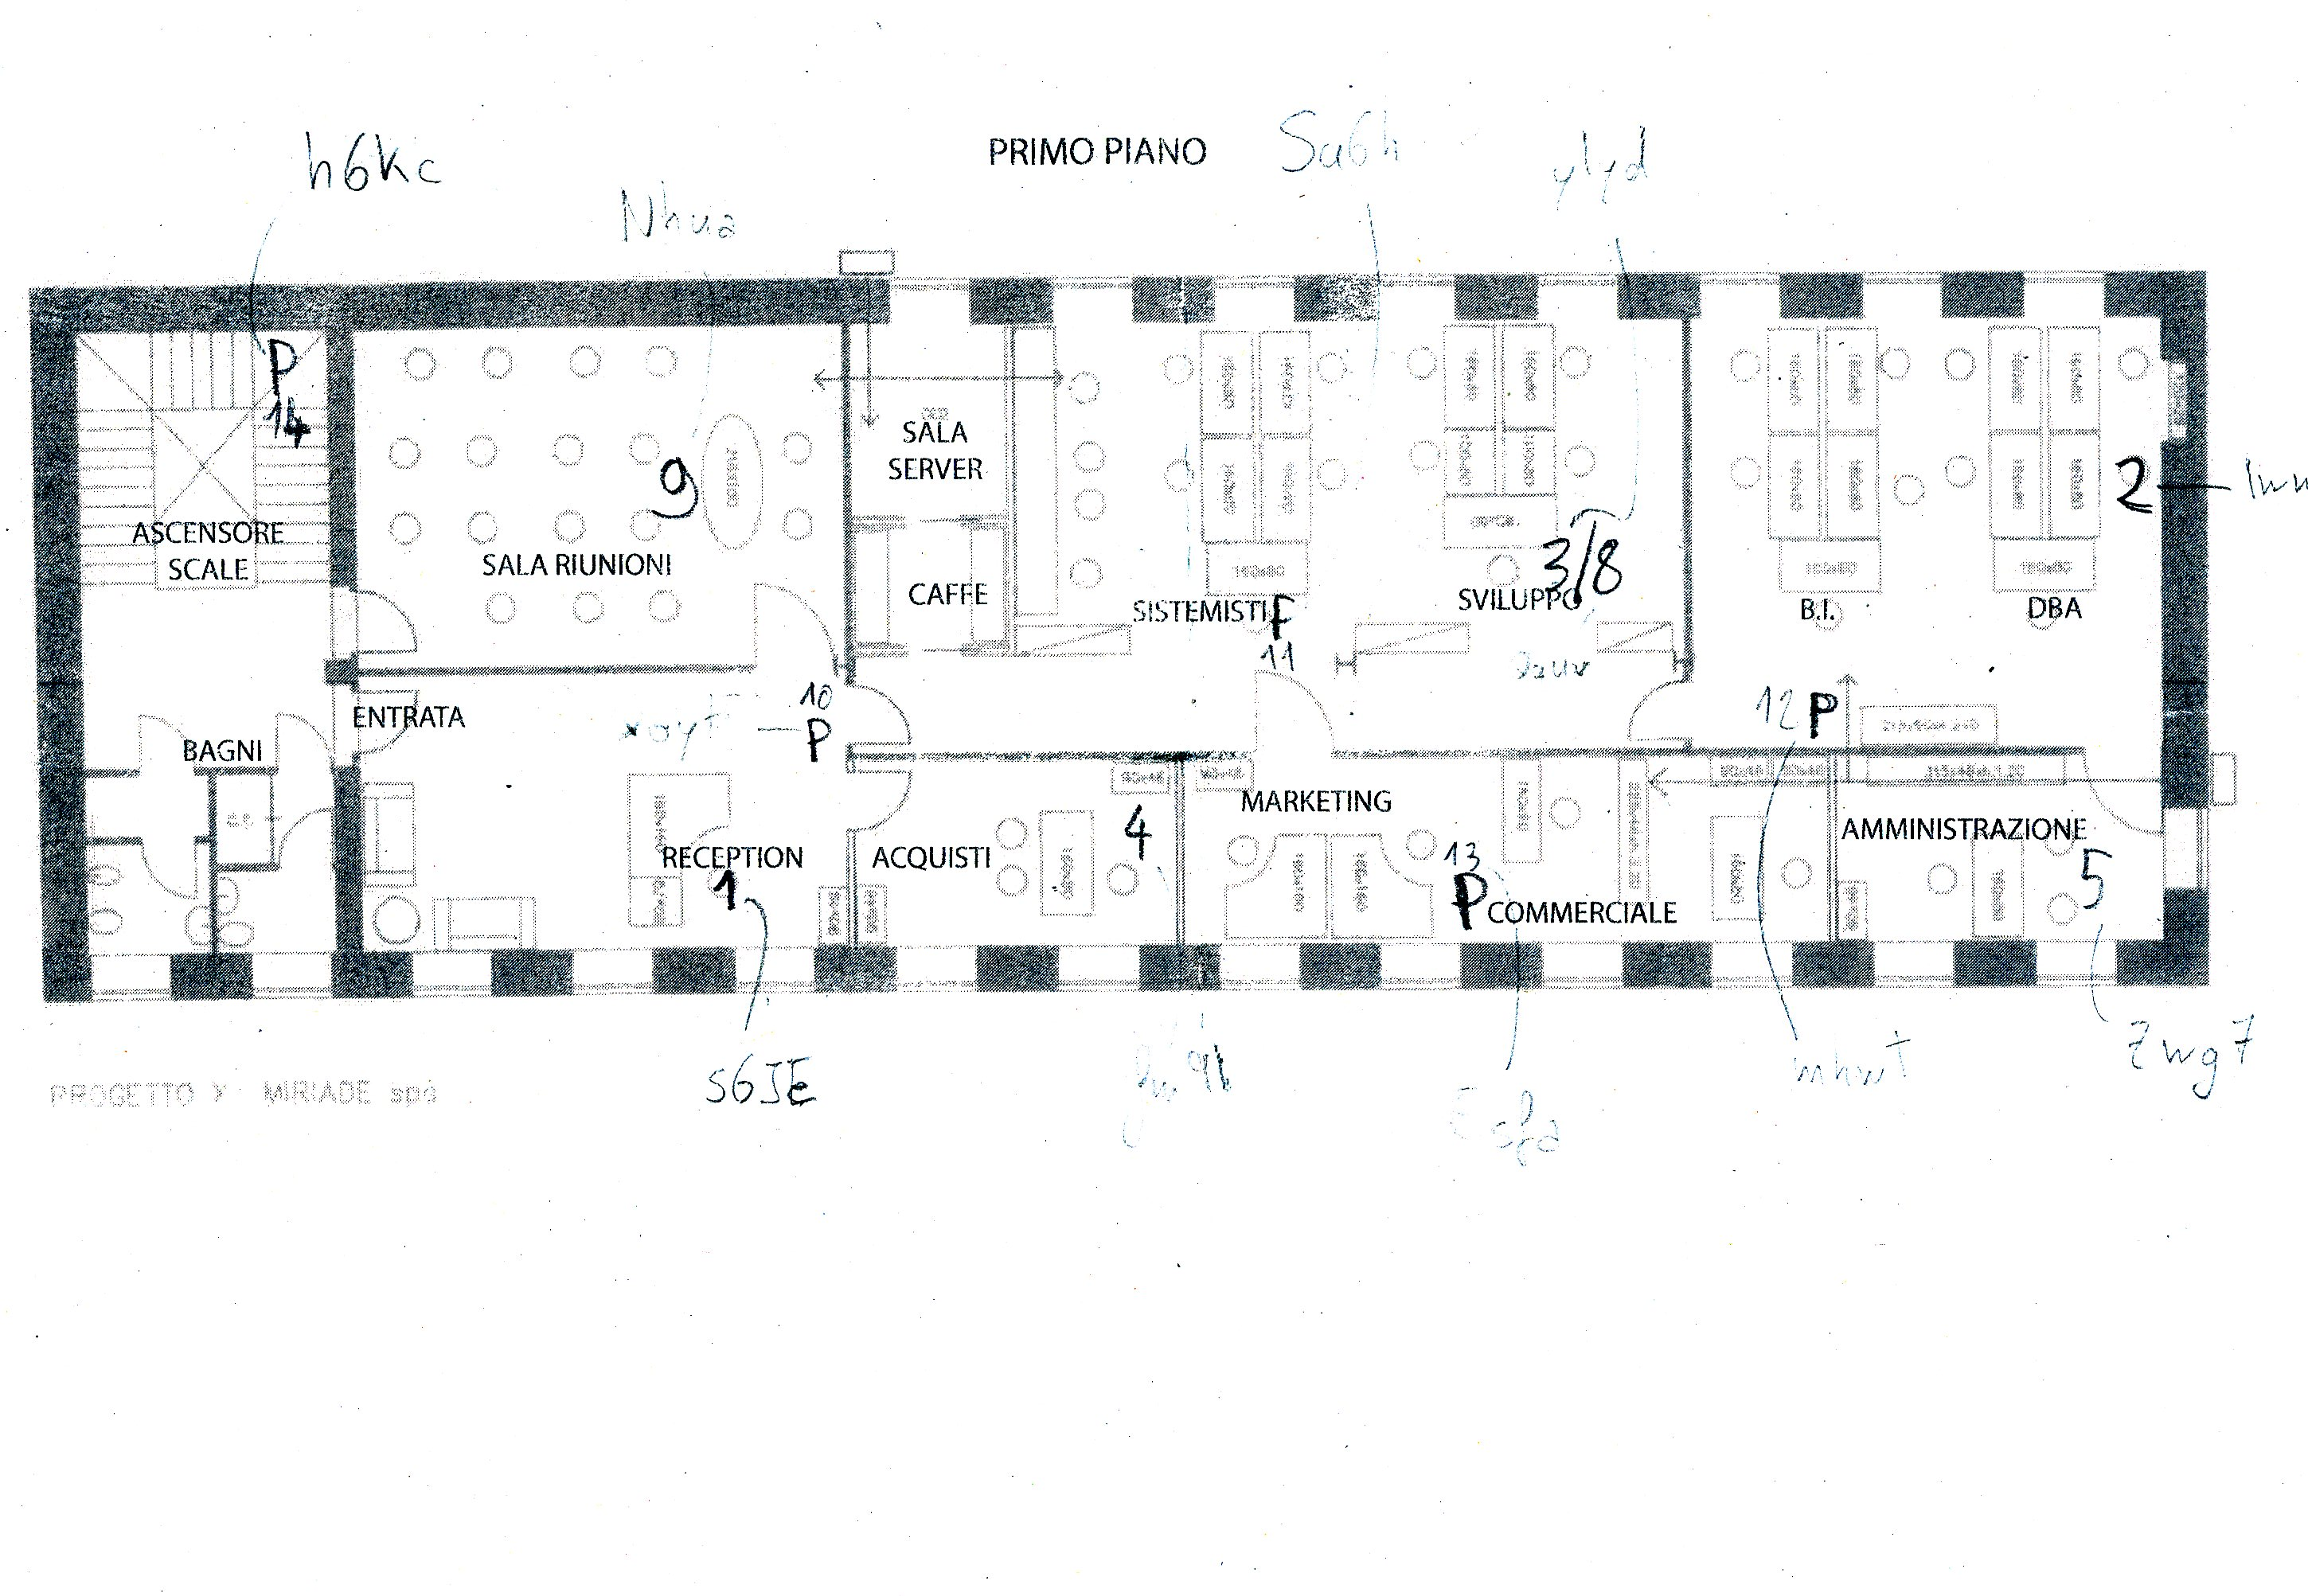
\includegraphics[scale=0.5]{planimetrie/Miriade1piano}  
				\caption{Planimetria del primo piano della sede di Miriade con la posizione dei beacon segnata}
		\end{figure}
		\begin{figure}[!h]
				\centering
				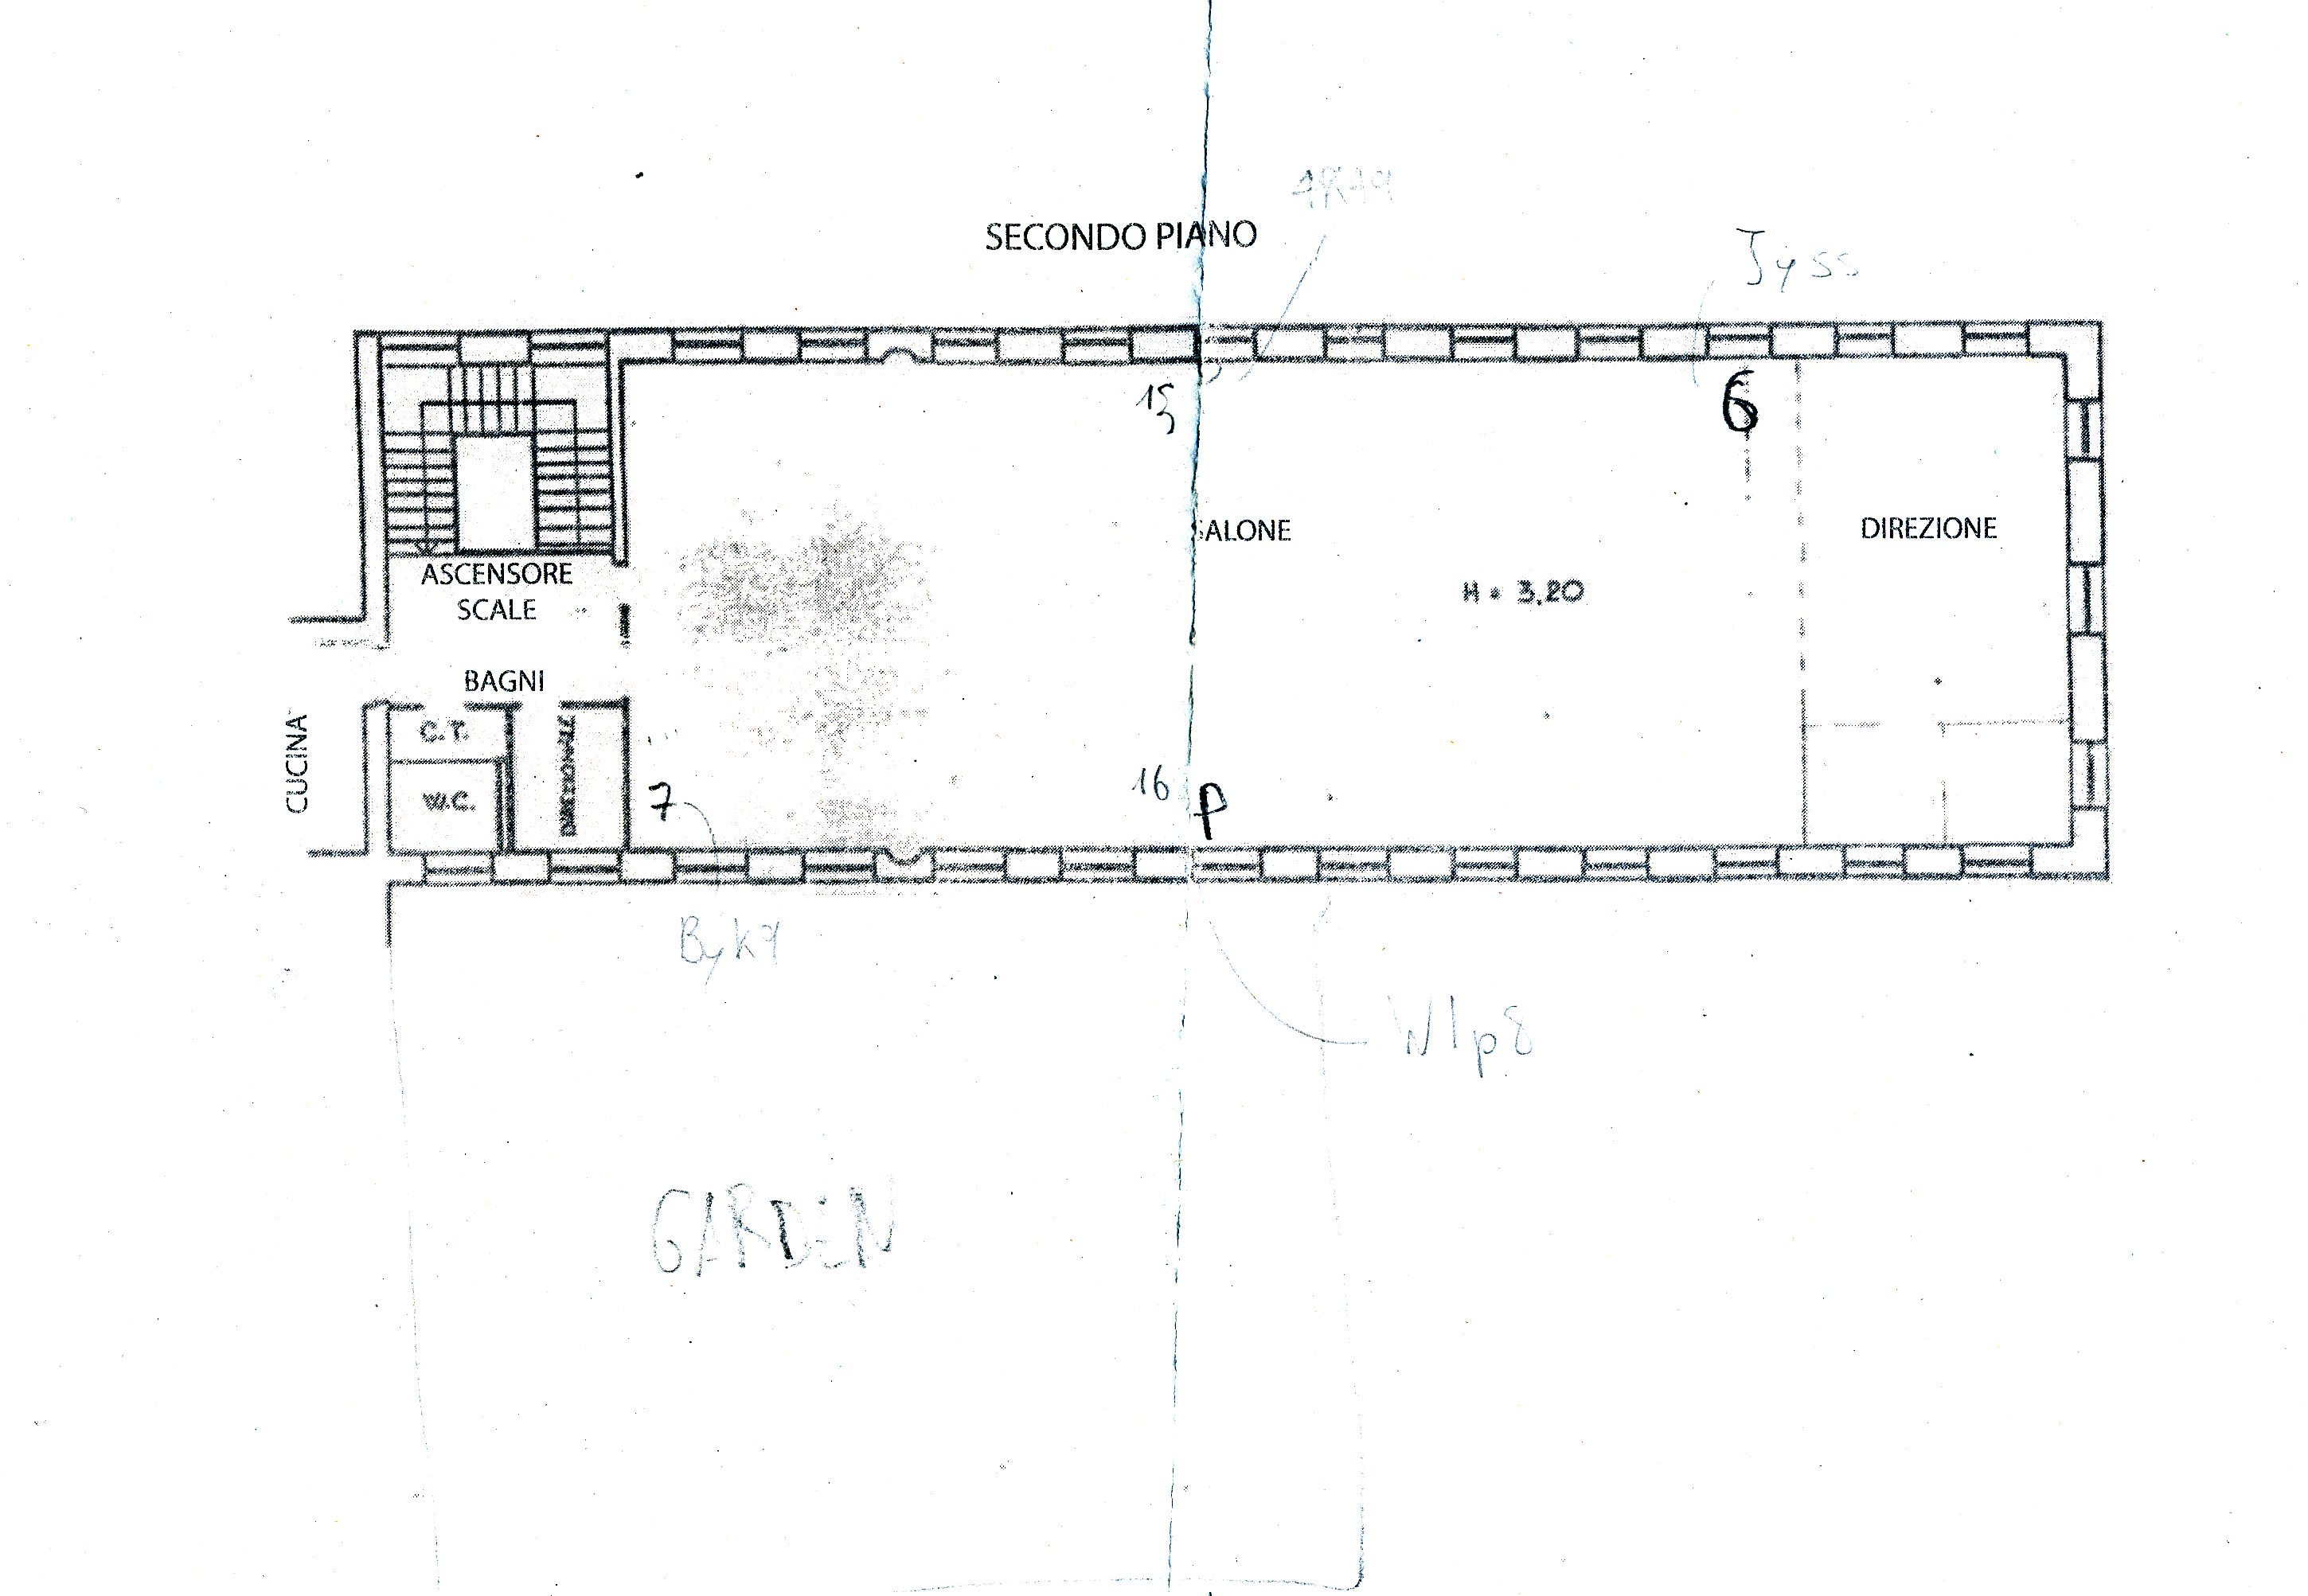
\includegraphics[scale=0.5]{planimetrie/Miriade2piano}  
				\caption{Planimetria del secondo piano della sede di Miriade con la posizione dei beacon segnata}
		\end{figure}
	
		\begin{tabella}{!{\VRule}l!{\VRule}l!{\VRule}l!{\VRule}l!{\VRule}l!{\VRule}l!{\VRule}}
			\intestazionesixcol{Numero beacon}{Major}{Minor}{Potenza (dBm)}{Intervallo (ms)}{Note posizione}
			1. & 0 & 0 & -20 & 150 & \\
			2. & 0 & 1 & -16 & 150 & \\
			3. & 0 & 2 & -20 & 150 & � il beacon sia della terza stazione sia dell'ottava \\
			4. & 0 & 3 & -30 & 150 & \\
			5. & 0 & 4 & -30 & 150 & \\
			6. & 0 & 5 & -30 & 350 & \\
			7. & 0 & 6 & -20 & 150 & \\
			9. & 0 & 8 & -20 & 150 & \\
			10. & 0 & 9 & -20 & 150 & \\
			11. & 0 & 10 & -30 & 150 & \\
			12. & 0 & 11 & -30 & 100 & \\
			13. & 0 & 12 & -30 & 350 & \\
			14. & 0 & 13 & -16 & 150 & \\
			15. & 0 & 14 & -20 & 350 & \\
			16. & 0 & 15 & -20 & 350 & \\
			\caption{Tabella con i dati dei beacon usati per il percorso}
		\end{tabella}
	
		\subsubsection{Esito della prova}
		La prova ha avuto successo, anche se la distanza a cui il beacon viene rilevato cambia in modo significativo a seconda del dispositivo; in particolare all'aumentare della versione di Android si ottiene una maggiore distanza in cui viene rilevato il beacon. Questo potrebbe causare problemi dentro a luoghi abbastanza piccoli, perch� porterebbe a rilevare dei beacon che in teoria dovrebbero essere distanti. Nel complesso comunque non dovrebbero esserci risultati che compromettano l'esecuzione del percorso.

\section{Valutazione del prodotto finale}
\label{valutazione}
%Qui daremo una valutazione del risultato finale in ambito SW, HW e UX (software, hardware e user experience), esaltando i pregi e riportando gli eventuali difetti da correggere
Per la progettazione di questo prodotto sono stati previsti degli obiettivi da raggiungere per ottenere il miglior risultato finale possibile. Durante la realizzazione del progetto essi sono in parte mutati, sia perché lo studio delle possibilità offerte da Android ha portato a soluzioni differenti, sia perché sono sorti alcuni problemi, come la mancanza di tempo o la maggior difficoltà incontrata nell'implementazione di una determinata caratteristica. In questa sezione verrà analizzato il prodotto, e quindi i relativi pregi e difetti, esaminandolo dal punto di vista del software, dell'hardware e della user experience.
	\subsection{Software}
		L'applicazione è divisa in vari package, ognuno con uno scopo preciso:
		\begin{itemize}
			\item ‘‘viewcontroller’’ contiene tutte le activity che gestiscono le GUI;
			\item ‘‘pathprogress’’ include le classi che gestiscono l'interazione con il GPS, quella con il Bluetooth e la memorizzazione dei risultati del percorso durante il suo svolgimento;
			\item ‘‘data’’ contiene le classi del Model e quelle specifiche per la loro costruzione;
			\item ‘‘datamanager’’ include le classi con lo scopo di ottenere i dati richiesti dal server o dal database locale, a seconda della polizza di cache usata;
			\item ‘‘urlrequest’’ contiene le classi responsabili della costruzione e dell'invocazione delle chiamate al server.
		\end{itemize}
		In questo modo è possibile verificare e modificare facilmente ogni passaggio di un'operazione.
		‘‘urlrequest’’ e ‘‘datamanager’’ contengono una struttura simile: è presente una gerarchia, in cui la cima è rappresentata da una classe astratta che svolge o gestisce le operazioni principali. Nel caso dell'‘‘urlrequest’’ tale classe crea ed esegue la chiamata in base ai parametri ricevuti, invece in ‘‘datamanager’’ essa gestisce le operazioni da fare in base alla politica di cache. Le classi derivate semplicemente definiscono i parametri e le azioni specifiche dell'operazione da gestire. Infine è presente una classe che funziona come una specie di interfaccia con il resto dell'applicazione, che contiene un metodo statico per ogni richiesta prevista. In questo modo si limitano le possibilità di commettere errori, perché gli esiti di ogni operazione sono facilmente verificabili e le classi responsabili degli errori eventuali sono subito identificabili.
		Come pattern per la notifica degli esiti delle richieste sono stati usati principalmente i listener, più che altro per comodità.
		Per quanto riguarda il GPS sono stati usati i Google Play Services, i più semplici da usare e anche i più recenti. Per le richieste al server è stata usata la libreria ‘‘Volley’’, più che sufficiente per l'uso che ne dovevamo fare. Per il rilevamento dei beacon è stato usato il framework messo a disposizione da Kontakt, semplice da implementare ma limitato, come spiegato tra le \hyperref[sec:libreria_beacon]{idee per il miglioramento dell'applicazione}.
		%TODO: aggiungere eventuali note per la parte di viewcontroller, ad esempio sul discorso delle classi Serializable oppure sulla gestione delle view, per esempio quando il formato dello schermo cambia
	\subsection{Hardware}
		L'applicazione non ha molti limiti per quanto riguarda il lato hardware, in cambio però richiede l'utilizzo di parecchi servizi. Innanzitutto occorre una connessione ad Internet per poter effettuare le richieste al server, sebbene tali chiamate abbiano una dimensione di pochi kB, e quindi anche una connessione debole dovrebbe essere sufficiente. È necessario poi utilizzare il GPS per rilevare la posizione dell'utente, in modo da informarlo se si trova vicino ad un edificio abilitato o no, e per mostrare l'elenco delle strutture più vicine; per ottenere un risultato accettabile è necessario avere una precisione elevata, perché ad esempio in città una bassa precisione potrebbe portare ad una lista degli edifici inconsistente, peggiorando la user experience. Infine è necessario usare il Bluetooth per rilevare i beacon.
		Il consumo della batteria rilevato durante i test è nella norma, ovvero è maggiore quando si esegue l'applicazione ma non eccessivo. Per far risparmiare batteria si potrebbe consigliare di disattivare il Bluetooth dopo aver finito di giocare un percorso e il GPS dopo aver trovato il percorso da giocare, anche se l'energia risparmiata è abbastanza poca.
		Le versioni di Android supportate dall'applicazione sono la 5 e le successive, perché sono quelle che supportano sufficientemente bene la lettura dei beacon. Nei dispositivi che usano la versione 6 di Android o una successiva è necessario abilitare i servizi per ogni singola applicazione, purtroppo non siamo riusciti a cercare una soluzione a questo ostacolo, che rappresenta un problema per la user experience, dato che il servizio non funziona anche se risulta acceso.
		Il tempo impiegato per rilevare il beacon varia a seconda del dispositivo: dalle prove che abbiamo fatto i risultati ottenuti vanno da cellulari che impiegano un secondo ad altri che invece ne impiegano anche 6 o 7. L'esito quindi è sufficiente per poter giocare un percorso, sebbene in certi casi bisogna aumentare la potenza del beacon per evitare che l'utente ci passi davanti senza fare in tempo a rilevarlo, ad esempio quando la stazione è situata in una zona di passaggio come un corridoio. Probabilmente cambiando la frequenza e la durata delle pause tra una ricerca e l'altra si possono ottenere risultati migliori.
		%TODO: vedere se aggiungere qualcosa relativa al viewcontroller, ad esempio se c'è qualcosa da segnalare per quanto riguarda la dimensione degli schermi
	\subsection{User experience}
		L'applicazione è strutturata in modo semplice, in modo da permettere all'utente di cominciare subito a giocare un percorso se si trova in un luogo abilitato. La prima pagina mostrata permette di cercare gli edifici più vicini, da cui poi è appunto possibile cominciare un percorso. Ogni GUI, a parte quelle che appaiono quando si gioca un percorso, presentano un menù da cui è possibile accedere a tutte le funzioni offerte dall'applicazione, fra cui la registrazione di un nuovo account, il login, il logout, le informazioni sul prodotto e sugli sviluppatori, la modifica dei dati del profilo e la ricerca degli edifici.
		Per giocare i percorsi non è necessario che l'utente abbia eseguito il login, se non vuole farlo semplicemente non può salvare il risultato ottenuto; viene comunque proposto all'utente di fare il login o di registrarsi quando finisce un percorso, in modo da poterne salvare l'esito. 
		Ogni volta che è necessario usare un servizio viene controllato se è attivo, in caso negativo l'utente viene invitato ad attivarlo; se non lo abilita non può andare avanti.
		Il pulsante per tornare indietro viene disabilitato quando l'utente inizia il percorso, in modo da impedirgli di rispondere ad una domanda a cui ha già risposto.
		Se viene rilevato un errore esso viene opportunamente segnalato, mostrando un messaggio all'utente; è però un sistema senz'altro migliorabile, ad esempio per quanto riguarda la visibilità e il messaggio che viene mostrato.
		La semplicità e l'uso immediato dell'applicazione sono uno dei punti fondamentali per la user experience, ma è possibile ottenere dei risultati ancora migliori, ad esempio \hyperref[sec:gestione_errori]{migliorando la gestione degli errori}\, come appunto è già stato detto, o \hyperref[sec:tutorial]{aggiungendo un tutorial introduttivo da mostrare al primo utilizzo}.
		%TODO: vedere se aggiungere qualcosa sulle GUI

\section{Idee per il miglioramento del prodotto finale}
\label{miglioramento}
%Qui metteremo le idee da proporre a Miriade per migliorare il prodotto, come l'interfaccia grafica per l'amministratore
Durante la progettazione del software il gruppo \AUTORE\ ha pensato ad alcune modifiche che, per mancanza di tempo, ha deciso di non applicare; l'implementazione di queste cambiamenti però porterebbe ad un miglioramento della qualità e dei servizi offerti dal prodotto. Di seguito saranno proposte queste modifiche, insieme ad una spiegazione dei miglioramenti che apporterebbero.
	\subsection{Interfaccia grafica per l'amministratore}
		Una componente che risulterebbe molto utile è l'interfaccia grafica per l'amministratore con cui inserire i dati da salvare nel server. I vantaggi principali sono due: si evitano i problemi di una formattazione errata dei dati da aggiungere, che possono presentarsi se i dati vengono inseriti direttamente a mano, e permette anche a responsabili che non conoscono gli oggetti JSON, il linguaggio SQL o la struttura del server di poter aggiungere dati senza preoccuparsi di provocare danni al sistema. Lo svantaggio è l'elevata mole di lavoro che richiede, in quanto sarebbe necessario creare un'interfaccia grafica per ogni tipo di dato da inserire, e in più richiederebbe una progettazione a sè per ottimizzarne l'usabilità.
	\label{libreria_beacon}
	\subsection{Utilizzo di librerie generiche per la lettura dei beacon}
		Le librerie Kontakt sono semplici da implementare e funzionano bene, hanno però il difetto di non poter interagire con tutti i tipi di beacon esistenti sul mercato. L'utilizzo di altre librerie, come ad esempio Android Beacon Library, dovrebbe permettere di risolvere questo problema.
	\label{gestione_errori}
	\subsection{Migliorare la gestione degli errori}
		Esiste già una gestione degli errori, ma è ancora grezza e migliorabile. In molti casi ad esempio viene mostrato un messaggio fisso, mentre sarebbe più utile visualizzare una delle spiegazioni contenute nella classe dell'errore, chiamata ServerError; in questo modo sarebbe più facile diversificare i messaggi mostrati a seconda del tipo di errore. Possono poi presentarsi due tipi di avvisi: il primo non permette di proseguire con l'operazione, ad esempio quando il percorso scelto non contiene delle stazioni perché non è ancora pronto, mentre il secondo permette comunque di andare avanti, ad esempio quando il percorso non contiene il titolo o un altro dato di secondaria importanza. Una buona gestione degli errori può aiutare ad individuare gli errori in tempi più brevi, e inoltre migliora la user experience, perché è meglio comunicare all'utente che c'è qualcosa di errato piuttosto di proseguire l'operazione inutilmente.
	\label{tutorial}
	\subsection{Aggiungere un tutorial introduttivo da mostrare al primo utilizzo}
		L'applicazione è semplice da utilizzare, ma alcuni passaggi potrebbero non essere immediati per chi la utilizza per la prima volta. Ad esempio è bene spiegare all'utente che la registrazione del profilo non è obbligatoria, o anche mostrargli dove può trovare una descrizione dell'applicazione. Per risolvere questo problema può essere utile mostrare un tutorial introduttivo al primo utilizzo, mentre per quelli successivi viene disabilitato ed eventualmente riabilitato dall'utente se lo desidera; in questo modo egli può comprendere più velocemente come funziona l'applicazione.
	\subsection{Aggiungere la schermata per mostrare i risultati delle singole prove}
		L'utente può vedere i risultati che ha ottenuto tramite un bottone dentro la GUI del profilo. Può essere utile e interessante permettergli di visualizzare anche i risultati delle singole prove per ogni percorso salvato, ad esempio trasformando la cella di ogni esito in un bottone cliccabile, da cui poi è possibile aprire una GUI simile in cui sono contenuti i risultati delle prove di quel percorso. Questi dati poi vengono già ricevuti quando si richiedono gli esiti dell'utente, quindi si tratterebbe solo di aggiungere un'Activity e di collegarla al resto dell'applicazione.
	\subsection{Aggiungere l'impossibilità di iniziare il percorso di un edificio distante dall'utente}
		Allo stato attuale l'utente può cominciare qualunque percorso anche se non si trova vicino all'edificio; ovviamente quando cerca il primo beacon non riesce a trovarlo. Per evitare questo inconveniente basterebbe sostituire il pulsante ??Inizia percorso?? con un messaggio in cui si avvisa l'utilizzatore che per iniziare il percorso deve recarsi in quell'edificio.
	\subsection{Aggiungere la possibilità di cambiare solo lo username}
		L'utente può già cambiare lo username e la password oppure solo la password, ma non può cambiare solo lo username. L'impedimento in realtà è dovuto soltanto alla GUI, perché il server prevede già la possibilità di effettuare la modifica dei dati solo con lo username e la vecchia password.
	\subsection{Aggiungere un'immagine dinamica alla proximity}
		La proximity per ora presenta solo un testo, che comunque dovrebbe migliorare la user experience. Verrebbe passato anche un valore percentuale, inzialmente pensato per poterlo rappresentare come una barretta o delle tacchette. In questo modo si dovrebbe dare un'idea all'utente di quanto si sta avvicinando o meno.
	\subsection{Migliorare la grafica dell'applicazione}
		Avere una bella grafica porta l'utente ad apprezzare di più l'applicazione, quindi sarà più disposto a provarla. Inoltre aiuta a convincere il possibile acquirente, dato che la grafica migliore aumenta
	\subsection{Lasso di tempo per poter far vedere i suggerimenti delle domande}
		Al momento attuale le domande contengono un pulsante per poter vedere un suggerimento, in modo da aiutare l'utente ad individuare la risposta corretta. Sarebbe più utile riuscire a far vedere quel pulsante dopo un certo lasso di tempo, così da poter inserire dei suggerimenti meno generici. Così facendo si aiuta l'utente a proseguire quando non riesce ad andare avanti. Sarebbe utile poi combinarlo con un algoritmo che calcola il punteggio anche in base al tempo impiegato dall'utente, in questo modo a lui non conviene aspettare di visualizzare il suggerimento se non è sicuro della risposta da dare.
	\subsection{Stazioni bonus}
		Un'aggiunta interessante potrebbe essere l'aggiunta di stazioni bonus, per assegnare dei punti bonus all'utente che riesce a completare la prova o semplicemente per mostrare un messaggio. In questo modo chi utilizza questa applicazione è portato a visitare anche i posti che non c'entrano con la tappa successiva, e in più è un incentivo a chi piace scoprire queste sorprese.


\end{document}